\newcommand{\imag}{{i\mkern1mu}}
\def \Leb {\mathrm{Leb}}

\def\proj{\mathrm{proj}}
\def\projM{\proj_{\mathcal{M}}}
\newcommand{\projR}[1]{\proj_{\mathcal{R}(#1)}}
\newcommand{\projsimpleR}{\proj_{\mathcal{R}}}
\newcommand{\projzero}[1]{\proj_{0, #1}}
\newcommand{\projone}[1]{\proj_{1, #1}}
\newcommand{\abs}[1]{| #1 |}
\def\Mclass{\mathcal{M}}
\def\Rclass{\mathcal{R}}

\def\pathmeas{\mathcal{P}(\mathcal{C})}

\def \rmA{\mathrm{A}}
\def \rmB{\mathrm{B}}
\def \rmC{\mathrm{C}}
\def \rmD{\mathrm{D}}


\def\KL{\mathrm{KL}}
\def\E{\mathbb{E}}
\def\N{\mathbb{N}}
\def\R{\mathbb{R}}
\def\P{\mathbb{P}}
\def\Pstar{\mathbb{P}^\star}
% \def\PSB{\mathbb{P}^\star}
\def\PSB{\mathbb{P}^\textup{SB}}
\def\pstar{p^\star}
\def\Pistar{\Pi^\star}
% \def\PiSB{\Pi^\star}
\def\PiSB{\Pi^\textup{SB}}
\def\Pihat{\hat{\Pi}}
\def\Phat{\hat{\P}}
\def\phat{\hat{p}}
\def\pistar{\pi^\star}
\def\Q{\mathbb{Q}}
\def\Qbridge{\mathbb{Q}_{|0,T}}
\def\Qhat{\hat{\Q}}
\def\qhat{\hat{q}}
\def\X{\mathcal{X}}

\newcommand{\schro}{Schr\"{o}dinger\xspace}


\def \argmin {\mathrm{argmin}}

\def \bfX {\mathbf{X}}
\def \bfT {\mathbf{T}}
\def \bfM {\mathbf{M}}
\def \bfZ {\mathbf{Z}}
\def \bfY {\mathbf{Y}}
\def \bfB {\mathbf{B}}

\def \nset {\mathbb{N}}
\def \rset {\mathbb{R}}

\def \Qbb {\mathbb{Q}}
\def \Pbb {\mathbb{P}}
\def \Mbb {\mathbb{M}}

\def \calR {\mathcal{R}}
\def \calC {\mathcal{C}}
\def \calM {\mathcal{M}}
\def \calP {\mathcal{P}}

\def \Leb {\mathrm{Leb}}

\def \rmd {\mathrm{d}}
\def \rmC {\mathrm{C}}

\def \msx {\mathsf{X}}
\def \msa {\mathsf{A}}

\def \vareps {\varepsilon}
\newcommand{\std}[1]{\scriptsize\rm$\pm$#1}
\newcommand{\gN}{\mathcal{N}}

\def \Id {\mathrm{Id}}

\def \Eproj {$\mathrm{E}$-projection ~}
\def \Mproj {$\mathrm{M}$-projection ~}


\newcommand \ccint[1]{[#1]}
\newcommand \coint[1]{[#1)}
\newcommand \ooint[1]{(#1)}
\newcommand \ensembleLigne[2]{\{ #1 \ : \ #2 \}}
\newcommand \expeLigne[2]{\mathbb{E}_{#1}[#2]}
\newcommand \CPELigne[3]{\mathbb{E}_{#1}[ #2 \ | \ #3 ]}
\newcommand \KLLigne[2]{\mathrm{KL}(#1|#2)}
\newcommand \normLigne[1]{\| #1 \|}

\newcommand{\valentin}[1]{\textcolor{red}{ {\small \ (Valentin)} #1}}
\newcommand{\ira}[1]{\textcolor{green}{ {\small \ (Ira)} #1}}
\newcommand{\andriy}[1]{\textcolor{blue}{ {\small \ (Andriy)} #1}}
\newcommand{\arnaud}[1]{\textcolor{orange}{ {\small \ (Arnaud)} #1}}

\newcommand{\citedcc}[2]{(\cite{#1}; #2)}

\DeclareMathOperator{\sech}{sech}
\DeclareMathOperator{\csch}{csch}


\newcommand{\vsra}{{\ensuremath{%
  \mathchoice{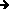
\includegraphics[height=1.1ex]{img/veryshortrightarrow.pdf}}
    {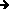
\includegraphics[height=1.1ex]{img/veryshortrightarrow.pdf}}
    {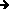
\includegraphics[height=.8ex]{img/veryshortrightarrow.pdf}}
    {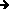
\includegraphics[height=.5ex]{img/veryshortrightarrow.pdf}}
}}}
\newcommand{\vsla}{{\ensuremath{%
  \mathchoice{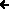
\includegraphics[height=1.1ex]{img/veryshortleftarrow.pdf}}
    {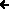
\includegraphics[height=1.1ex]{img/veryshortleftarrow.pdf}}
    {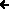
\includegraphics[height=.8ex]{img/veryshortleftarrow.pdf}}
    {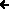
\includegraphics[height=.5ex]{img/veryshortleftarrow.pdf}}
}}}

\newcommand\vvsra{\stackrel{\mathclap{\vsra n}}{v}}
\def \rmD {\mathrm{D}}
\def \Lparam {\mathrm{L}}
\def \Lnonparam {\mathcal{L}}


%%% Local Variables:
%%% mode: latex
%%% TeX-master: "main"
%%% End:
